%\title{Article HW Template}

\documentclass[12pt]{article}
\usepackage[paper=a4paper,top=1in, bottom=1in, right=1in, left=.7in]{geometry}
\usepackage{amsthm, amssymb, amsfonts, amsmath}
\usepackage{graphicx}
\usepackage{tikz}
\usetikzlibrary{calc,shapes}
\usepackage{enumitem}
\usepackage{mathtools}
\usepackage{mathrsfs}
\usepackage{tikz-cd}
\usepackage{hyperref, mathabx}

\newcommand{\boxitem}[2]{\vspace{.55cm}
	\item[#1]
	\leavevmode
	\strut
	\vadjust{%%
		\noindent
		\raisebox{\dimexpr\dp\strutbox+\ht\strutbox+1ex}[0pt][0pt]{\tikzmark{bl}}}%%
	#2
	
	\leavevmode
	\vadjust{%
		\noindent
		\hspace*{\dimexpr\textwidth+1ex}\tikzmark{br}}%%
	
	\tikz[overlay,remember picture]{\draw[black]
		(bl) rectangle
		(br);}}

\newcommand{\tikzmark}[1]{\tikz[overlay,remember picture] \node (#1) {};}

\newcommand{\R}{\mathbb{R}}
\newcommand{\Q}{\mathbb{Q}}
\newcommand{\Z}{\mathbb{Z}}
\newcommand{\N}{\mathbb{N}}
\newcommand{\p}{\mathbb{P}}
\newcommand{\E}{\mathbb{E}}
\newtheorem*{lemma}{Lemma}
\newtheorem{llemma}{Lemma}
\newtheorem*{theorem}{Theorem}
\newtheorem*{prop}{Proposition}

\begin{document}
	\null\hfill\begin{tabular}[t]{r@{}}
		Nikolas Mavrogeneiadis - 161014\\
		gravitorious \\
		University Of West Attica \\
		Department of Informatics and Computer Engineering\\
		Professor: Panagiotis Rouvelas\\
		\today
	\end{tabular}
	\\
	\centerline{\scshape{Graph Theory-Exercise Set 1}}
	
	\begin{enumerate}[listparindent=1.5em,
		parsep = 0pt]
		
	\boxitem{1.}{
		Prove that at least two vertices have the same degree in any simple graph with $n(vertices)>2$.
	}
		\underline{Proof:}
		Let $G(V,E)$ be a simple graph that for every pair of vertices $v_1$ and $v_2$ we have that $d(v1) \neq d(v2)$ where $d(v)$ is the degree of vertex $v$. Then, each vertex has a degree from the set $\{0, 1, 2, ..., n-1\}$. This means that there is a vertex with degree 0 and vertex with degree n - 1. But this is a contradiction.
		
	\boxitem{2.}{
		Let H be subgraph of G. Which of the following statements is correct? \\
		$i) d(G) \geq d(H)$ \\
		$ii) D(G) \geq D(H)$ \\
	}
		\underline{Proof:}
		For the $i)$ it is easy to find a counterexample. Let G with $d(G) = 1$ and there are only one vertex $v_1$ with this degree. We can delete this vertex and the new subgraph H will have $d(H) = 2$. \\
		\begin{figure}[h]
			\centering
			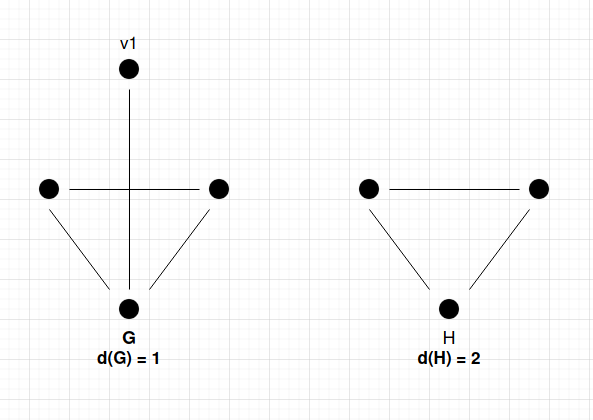
\includegraphics[width=0.55\textwidth]{pic1}
			\caption{A counterexample}
			\label{fig:mesh1}
		\end{figure}\\
		For the $ii)$ assume that exists $G(V,E)$ and its subgraph $H(\hat{V}, \hat{E})$ with $D(G) < D(H)$. This means that H contains an edge that G not. But this is a contradiction because $\hat{E} \subseteq E$.
		
	\boxitem{3.}{
		Prove that doesn't exist a 2k-regular graph with bridge.
	}
	\underline{Proof:} Assume that exists a 2k-regular graph with bridge. This means that each vertex has an even degree. If we delete the bridge edge, then we will have two components. Each of these has exactly one vertex with odd degree and with the rest having even degree. This means that the sum of degrees of all vertices for each component is odd number. This is a contradiction because we know that the sum of degrees is an even number.
	
	\boxitem{4.}{
		Prove that for every finite graph G, exists $m>0$ with $G^{m+1} = G^{m}$.
	}
	\underline{Proof:} Let diameter(d) be the maximum distance of G between any pair of vertices. Let the pair of vertices $(v_{1}, v_{2})$ be that with the maximum distance. Then it is easy to see that $G^{d}$ is a complete graph because if it isn't, the path from $v_{1}$ to $v_{2}$ is more than one, so d wasn't the maximum distance. A contradiction. Let $m:=d$. Then $G^{m+1}$ is the same complete graph. So $G^{m} = G^{m+1}$.
	
	\boxitem{5.}{
		Prove that for every simple graph G(V,E) with $n = |V|$ and $d(G)\geq\frac{n-1}{2}$ is connected.
	}
	\underline{Proof:} Suppose that G is not connected. Then G has at least two components. Each of these have at least one vertex with degree $\frac{n-1}{2}$. Now counting all the vertices of graph (including the two vertices) we see that $|V| = \frac{n-1}{2} + \frac{n-1}{2} + 1 + 1 = n+1$. A contradiction.
	
	
		
		
		
	
		
	\end{enumerate}
\end{document}
